% Søylediagram (pgfplots): HDOs sluttevaluering per kravområde.
% Tallene er gjennomsnitt av respondentene; kilden er tabell~\ref{tab:hdo-eval-full} i vedlegg~\ref{app:hdo-eval}.
% Brukes typisk via \texttt{figures/hdo-eval-sammendrag.tex} i hovedteksten.
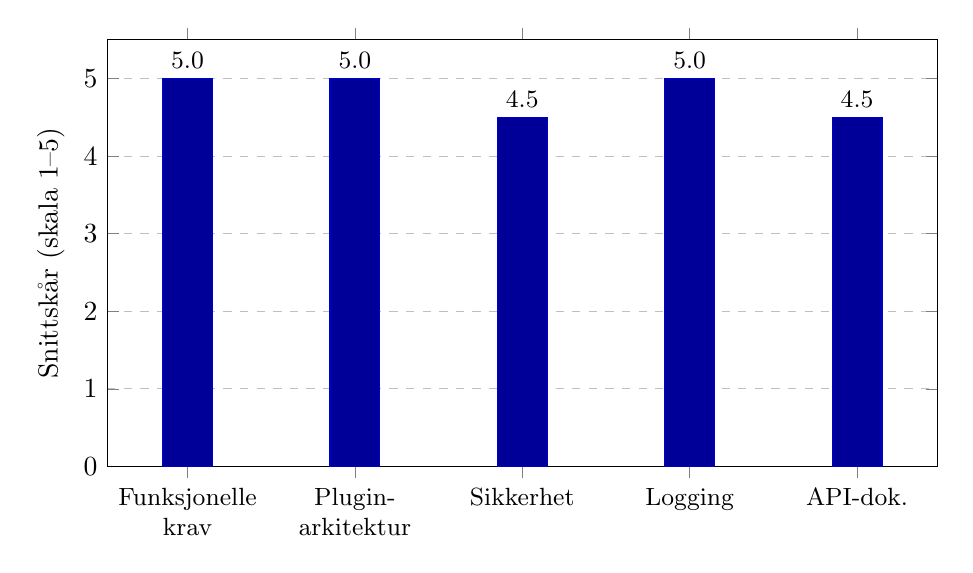
\begin{tikzpicture}
    \begin{axis}[
        width=\linewidth,
        height=7cm,
        ybar,
        bar width=18pt,
        ymin=0,
        ymax=5.5,
        ytick={0,1,2,3,4,5},
        ylabel={Snittskår (skala 1--5)},
        symbolic x coords={
            {Funksjonelle\\krav},
            {Plugin-\\arkitektur},
            {Sikkerhet},
            {Logging},
            {API-dok.},
            {Samlet\\leveranse}
        },
        xtick=data,
        xticklabel style={
            align=center,
            font=\small,
            text width=2cm
        },
        nodes near coords,
        nodes near coords style={font=\small},
        every node near coord/.append style={
            /pgf/number format/.cd,
            fixed,
            fixed zerofill,
            precision=1
        },
        enlarge x limits=0.12,
        ymajorgrids=true,
        grid style=dashed,
    ]
        \addplot[
            fill=blue!60!black,
            draw=blue!80!black
        ] coordinates {
            ({Funksjonelle\\krav},5.0)
            ({Plugin-\\arkitektur},5.0)
            ({Sikkerhet},4.5)
            ({Logging},5.0)
            ({API-dok.},4.5)
        };
    \end{axis}
\end{tikzpicture}
